\subsubsection{IT}
Le département de l'IT est le gardien principal de toutes les tâches IT communes comme:
\begin{itemize}
  \item La gestion des environnements virtuels. (cloud ou serveur physique).
  \item La gestion de l'automatisation de processus de CI interne.
  \item La gestion des licences des applications payantes (OS, applications).
  \item La gestion des appareils, périphériques, les ordinateurs portables,
  \item L'architecture, méthodologies et règles régissant l'utilisation et le stockage des données.
  \item L'administration de systèmes: la configuration, gestion, entretien et dépannage des environnements
  informatiques multi-utilisateurs (cloud ou physique).
  \item  La gestion ou l'aide aux autres départements avec la culture et pratiques DevOps.
\end{itemize}

Aussi, l'équipe d'IT de Bonitasoft gère d'autres projets comme:
\begin{itemize}
  \item Salesforce: depuis la création des use cases jusqu'à la mise en production en garantissant la gouvernance du système avec une approche DevOps.
  \item BCD: c'est une solution fournie pour utiliser les bonnes pratiques DevOps pour la livraison continue (CI) d'une application Bonita.
\end{itemize}

L'équipe est composée de quatre personnes, dont je fais partie.

\begin{figure}[h]
  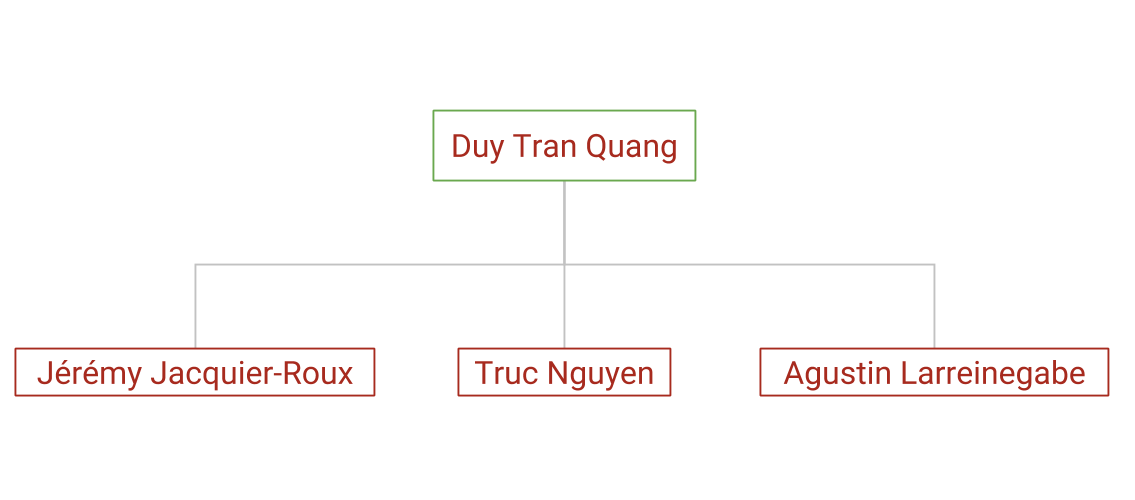
\includegraphics[width=\textwidth,keepaspectratio]{it_team.png}
   \caption{Organigramme.}
   \label{figure:organigrame}
\end{figure}
